\documentclass[journal,12pt,onecolumn]{IEEEtran}
\usepackage{amsmath,amssymb,amsfonts,amsthm}
\usepackage{graphicx}
\usepackage{enumitem}
\usepackage[breaklinks=true]{hyperref}
\usepackage{caption}

\newtheorem{problem}{Problem}
\renewcommand{\thefigure}{\theenumi}
\renewcommand{\thetable}{\theenumi}

\newcommand{\myvec}[1]{\begin{pmatrix}#1\end{pmatrix}}


\begin{document}

\title{GATE XE 2015}
\author{AI25BTECH11003 - Bhavesh Gaikwad}
\maketitle

%-----------GA--------------
\section*{General Aptitude}
\vspace{1cm}
\begin{enumerate}[label=\arabic*)]

\item Choose the most appropriate word from the options given below to complete the following sentence.\\
The principal presented the chief guest with a \_\_\_\_\_\_\_ as token of appreciation.  
\hfill\raisebox{-1.5ex}{(GATE 2015 XE)} \\
\vspace{0.2cm}
\begin{enumerate}[label=\alph*)]
\item momento
\item memento
\item momentum
\item moment
\end{enumerate}

\vspace{0.5cm}

\item Choose the appropriate word/phrase to complete the following sentence: 
Frogs \_\_\_\_\_.  
\hfill\raisebox{-3.5ex}{(GATE 2015 XE)} \\

\vspace{0.2cm}
\begin{enumerate}[label=\alph*)]
\item croak
\item roar
\item hiss
\item patter
\end{enumerate}

\vspace{0.5cm}

\item Choose the word most similar in meaning to the given word: \textbf{Educe}  
\hfill\raisebox{-2.5ex}{(GATE 2015 XE)} \\
\vspace{0.2cm}
\begin{enumerate}[label=\alph*)]
\item Exert
\item Educate
\item Extract
\item Extend
\end{enumerate}

\vspace{0.5cm}

\item Operators, $\diamondsuit$ and $\square$, are defined by:  
$a\diamondsuit b = \frac{a-b}{a+b}$ ; \quad $a\square b = \frac{a+b}{a-b} = ab$.  
Find the value of $(6\diamondsuit 6) \square (6\diamondsuit 6)$.
\vspace{0.2cm}
\hfill\raisebox{-2.5ex}{(GATE 2015 XE)} \\

\begin{enumerate}[label=\alph*)]
\item $-2$
\item $-1$
\item $1$
\item $2$
\end{enumerate}

\vspace{0.5cm}

\item If $\log_x \left(\frac{5}{7}\right) = -\frac{1}{3}$, then the value of $x$ is  

\vspace{0.2cm}
\begin{enumerate}[label=\alph*)]
\item $\frac{343}{125}$
\vspace{0.1cm}
\item $\frac{125}{343}$
\vspace{0.1cm}
\item $\frac{-25}{49}$
\vspace{0.1cm}
\item $\frac{-49}{25}$
\end{enumerate}

\vspace{0.5cm}

\item The following sentence has a part underlined. Choose the most effective alternative:  

\emph{Tuberculosis, together with its effects, ranks one of the leading causes of death in India.}  
\hfill\raisebox{-2.5ex}{(GATE 2015 XE)} \\

\vspace{0.2cm}
\begin{enumerate}[label=\alph*)]
\item ranks as one of the leading causes of death
\item rank as one of the leading causes of death
\item has the rank of one of the leading causes of death
\item are one of the leading causes of death
\end{enumerate}

\vspace{0.5cm}

\item Read the paragraph and choose the correct statement.  

Climate change has reduced human security and threatened human well-being. An ignored reality is that human security largely depends upon environmental security. But on the contrary, human progress seems contradictory to environmental security.  
\hfill\raisebox{-2.5ex}{(GATE 2015 XE)} \\

\vspace{0.2cm}
\begin{enumerate}[label=\alph*)]
\item Human progress and security are positively associated with environmental security.
\item Human progress is contradictory to environmental security.
\item Human security is contradictory to environmental security.
\item Human progress depends upon environmental security.
\end{enumerate}

\vspace{0.5cm}

\item Fill in the missing value:
\begin{figure}[htbp]
  \centering
  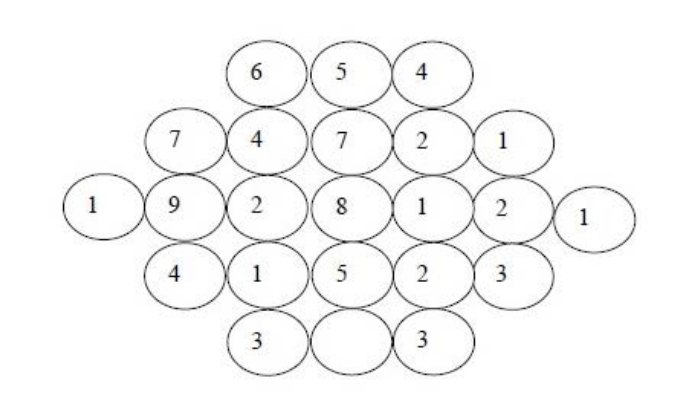
\includegraphics[width=.6\linewidth]{figs/GA/fig1.png}
  \caption{Puzzle}
  \label{GA/fig1}
\end{figure}

\hfill\raisebox{-7.5ex}{(GATE 2015 XE)} \\


\vspace{0.5cm}

\item A cube of side $3$ units is formed using smaller cubes of side $1$ unit. Find the proportion of faces visible to those NOT visible.
\hfill\raisebox{-2.5ex}{(GATE 2015 XE)} \\

\vspace{0.2cm}
\begin{enumerate}[label=\alph*)]
\item $1:4$
\item $1:3$
\item $1:2$
\item $2:3$
\end{enumerate}

\vspace{0.5cm}

\item Humpty Dumpty sits on a wall every day while having lunch. The wall sometimes breaks. If the wall breaks, the person falls.

Which statement is logically valid?  

\vspace{0.2cm}
\begin{enumerate}[label=\alph*)]
\item Humpty Dumpty always falls while having lunch
\item Humpty Dumpty does not fall sometimes while having lunch
\item Humpty Dumpty never falls during dinner
\item When Humpty Dumpty does not sit on the wall, the wall does not break
\end{enumerate}

\end{enumerate}
\vspace{3\baselineskip}
\begin{center}
    \item[\textbf{END OF SECTION- GA}]
\end{center}

%----------------SECTION-A----------------------

\newpage
\section*{Engineering Mathematics}
\vspace{1cm}

\begin{enumerate}[label=\arabic*)]

\item Considering the matrix
$\myvec{ 0 & -1 & 2 \\ 1 & 0 & 3 \\ -2 & -3 & 0}$
which one of the following statements is INCORRECT?
\vspace{0.2cm}
\hfill\raisebox{0.5ex}{(GATE 2015 XE)} \\

\begin{enumerate}[label=\alph*)]
\item One of its eigenvalues is zero.
\item It has two purely imaginary eigenvalues.
\item It has a non-zero real eigenvalue.
\item The sum of its eigenvalues is zero.
\end{enumerate}

\vspace{0.5cm}

\item The value of $x$ where $f(x) = \sin{x} + \cos{x}$ attains a minimum in $0 \le x \le 2\pi$ is \_\_\_\_\_\_\_\_
\vspace{0.2cm}
\hfill\raisebox{-2.5ex}{(GATE 2015 XE)} \\

\vspace{0.5cm}

\item The radius of convergence of $\sum_{n=0}^\infty \frac{(x-3)^n}{3^n\,n!}$  
\hfill\raisebox{-2.5ex}{(GATE 2015 XE)} \\

\vspace{0.2cm}
\begin{enumerate}[label=\alph*)]
\item zero
\item 1
\item 3
\item $\infty$
\end{enumerate}

\vspace{0.5cm}

\item For complex $k$ and $z$, $(z+k)^2$ is analytic  
\hfill\raisebox{-2.5ex}{(GATE 2015 XE)} \\

\vspace{0.2cm}
\begin{enumerate}[label=\alph*)]
\item for all $k$
\item only when the imaginary part of $k$ is zero
\item only when the real part of $k$ is zero
\item only when $k=0$
\end{enumerate}

\vspace{0.5cm}

\item The divergence of $\mathbf{v} = 2x\,\mathbf{i} + 2y\,\mathbf{j} + 2z\,\mathbf{k}$ at $(1,1,1)$ is \_\_\_\_\_\_\_\_\_\_
\hfill\raisebox{-2.5ex}{(GATE 2015 XE)} \\
\vspace{0.5cm}

\item The type of the differential equation  
$(1-x)\frac{d^3 y}{dx^3} + \sqrt{1+\left(\frac{dy}{dx}\right)^2} + 5y = \cos{x}$
\hfill\raisebox{-2.5ex}{(GATE 2015 XE)} \\

\vspace{0.2cm}
\begin{enumerate}[label=\alph*)]
\item linear and first order
\item non-linear and first order
\item linear and third order
\item non-linear and third order
\end{enumerate}

\newpage

\item A box has 10 bulbs, 2 defective, drawn without replacement. Probability both are NOT defective:
\vspace{0.2cm}
\hfill\raisebox{-2.5ex}{(GATE 2015 XE)} \\

\begin{enumerate}[label=\alph*)]
\item $\frac{8}{45}$
\vspace{0.1cm}
\item $\frac{28}{45}$
\vspace{0.1cm}
\item $\frac{16}{25}$
\vspace{0.1cm}
\item $\frac{4}{5}$
\end{enumerate}

\vspace{0.5cm}

\item The limit value:
$\lim_{x\to\infty} \frac{x - \sin{x}}{x + \sin{x}} + \frac{\ln{x}}{x}$
\hfill\raisebox{-2.5ex}{(GATE 2015 XE)} \\

\vspace{0.2cm}
\begin{enumerate}[label=\alph*)]
\item zero
\item 1
\item 2
\item $\infty$
\end{enumerate}

\vspace{0.5cm}

\item The $A_0$ of Fourier series of $f(x)=x^2$ over $0 \le x \le 2\pi$ is  
\hfill\raisebox{-2.5ex}{(GATE 2015 XE)} \\

\vspace{0.2cm}
\begin{enumerate}[label=\alph*)]
\item $\frac{4\pi^2}{3}$
\item $\frac{2\pi^2}{3}$
\item $\frac{\pi^2}{3}$
\item $\frac{\pi^2}{6}$
\end{enumerate}

\vspace{0.5cm}

\item The general solution $y(x)$ for  
$x\,\frac{d^2y}{dx^2} + \frac{dy}{dx} - 1 = 0$
is  
\hfill\raisebox{-2.5ex}{(GATE 2015 XE)} \\

\vspace{0.2cm}
\begin{enumerate}[label=\alph*)]
\item $\frac{C_1x^2}{2} + 2x + C_2$
\vspace{0.1cm}
\item $\frac{C_1x^2}{2} - x + C_2$
\vspace{0.1cm}
\item $\frac{C_1x^2}{2} + x + C_2$
\vspace{0.1cm}
\item $\frac{C_1x^2}{2} - 2x + C_2$
\end{enumerate}

\vspace{0.5cm}

\item Minimum Newton–Raphson iterations to get $\sqrt{28}$ correct to $3$ decimals starting at $5$: \_\_\_\_
\hfill\raisebox{-3.5ex}{(GATE 2015 XE)} \\

\end{enumerate}

\vspace{3\baselineskip}
\begin{center}
    \item[\textbf{END OF SECTION- A}]
\end{center}


%-----------------SECTION-B-----------------
\newpage

\section*{Fluid Mechanics}
\vspace{1cm}
\begin{enumerate}[label=\arabic*)]

% Q22
\item The gap $\delta$ between two concentric cylinders, each of height $h$, is filled with an oil. The torque required to rotate the inner cylinder at angular velocity $\omega$ against the fixed outer cylinder is $T$. The diameter of the inner cylinder is $d$ and $\delta \ll d$. The dynamic viscosity of the oil is  
\hfill\raisebox{-2.5ex}{(GATE 2015 XE)} \\

\vspace{0.2cm}
\begin{enumerate}[label=\alph*)]
\item $\dfrac{4\pi \delta T}{d^3 \omega h}$
\vspace{0.1cm}
\item $\dfrac{4\delta T}{\pi d^3 \omega h}$
\vspace{0.1cm}
\item $\dfrac{4\pi \delta T}{d^2 \omega h^2}$
\vspace{0.1cm}
\item $\dfrac{4\delta T}{\pi d \omega h^3}$
\end{enumerate}
\vspace{0.5cm}

% Q23 (image: fig1)
\item Water is retained against a sluice gate in the form of a circular segment as shown in the figure. If $\rho$ and $g$ are the density of water and gravitational acceleration, respectively, the upward force exerted by the gate on the water per unit depth perpendicular to the plane of the figure is  

\begin{figure}[htbp]
  \centering
  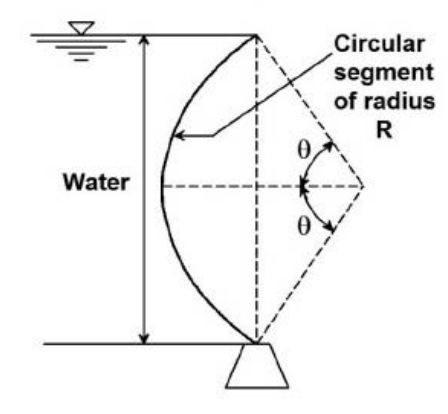
\includegraphics[width=.6\linewidth]{figs/B/fig1.png} 
  \caption{Diagram}
  \label{B/fig1}
\end{figure}


\hfill\raisebox{-2.5ex}{(GATE 2015 XE)} \\
\vspace{0.2cm}
\begin{enumerate}[label=\alph*)]
\item $\rho R^2 \left(\theta - \frac{1}{2} \sin 2\theta \right) g$
\item $\rho R^2 \left(\cos^2 \theta - \frac12 \sin \theta \right) g$
\item $\rho R^2 \left(\cos \theta - \frac12 \sin \theta \right) g$
\item $\rho R^2 \left(\cos^2 \theta - \frac12 \sin^2 \theta \right) g$
\end{enumerate}

\newpage

% Q24
\item A two-dimensional velocity field is given by  
$\vec{V} = 10(y^3 - x^2 y) \, \mathbf{i} + 2C x y^2 \, \mathbf{j}$, where $\mathbf{i}$ and $\mathbf{j}$ are unit vectors in $x$ and $y$ directions, respectively. If the flow is incompressible, the constant $C$ should be  

\hfill\raisebox{-2.5ex}{(GATE 2015 XE)} \\
\vspace{0.2cm}
\begin{enumerate}[label=\alph*)]
\item $-10$
\item $0$
\item $5$
\item $10$
\end{enumerate}
\vspace{0.5cm}

% Q25
\item Let $\vec{V}$ and $T$ denote the velocity vector and temperature in a flow field. The rate of change of temperature experienced by a fluid particle at $(x_1, y_1, z_1)$ at time $t_1$ is $2.5 \ ^\circ\mathrm{C/s}$. The rate of change of temperature at the fixed point $(x_1, y_1, z_1)$ at time $t_1$ is $4.8 \ ^\circ\mathrm{C/s}$. The quantity $\vec{V} \cdot \nabla T$ at $(x_1, y_1, z_1, t_1)$ in $^\circ\mathrm{C/s}$ is \_\_\_\_
\hfill\raisebox{-1.5ex}{(GATE 2015 XE)} \\

\vspace{0.5cm}

% Q26
\item In a simple Couette flow apparatus, the gap $h$ between parallel plates is filled with a liquid of density $\rho$ and dynamic viscosity $\mu$. One plate is dragged at velocity $U$ parallel to itself, the other plate is fixed. The magnitude of vorticity at any point is  

\hfill\raisebox{-2.5ex}{(GATE 2015 XE)} \\
\vspace{0.2cm}
\begin{enumerate}[label=\alph*)]
\item $\frac{\mu}{\rho h^2}$
\vspace{0.1cm}
\item $0$
\item $\dfrac{1}{h^2} \sqrt{\frac{\mu \nu h}{\rho}}$
\vspace{0.1cm}
\item $\frac{U}{h}$
\end{enumerate}
\vspace{0.5cm}

% Q27 (image: fig2)
\item An open glass capillary tube of $2\,\mathrm{mm}$ bore is lowered into a cistern of mercury ($\rho=13600$ kg/m$^3$). Contact angle between mercury and glass is $140^\circ$, surface tension coefficient $=0.484$ N/m, $g=9.81$ m/s$^2$. The depression of mercury in the tube, in mm, is \_\_\_\_

\begin{figure}[htbp]
  \centering
  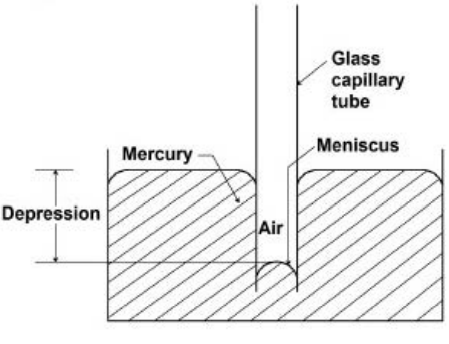
\includegraphics[width=.38\linewidth]{figs/B/fig2.png} 
  \caption{Diagram}
  \label{B/fig2}
\end{figure}

\hfill\raisebox{-2.5ex}{(GATE 2015 XE)} \\

\newpage

% Q28
\item Consider a combined forced-free vortex. The central region radius $R$, angular velocity $\omega$ is a forced vortex, the rest is free vortex. Pressure at the edge is $p_0$. Fluid density is $\rho$. The pressure at the center is  
\hfill\raisebox{-2.5ex}{(GATE 2015 XE)} \\

\vspace{0.2cm}
\begin{enumerate}[label=\alph*)]
\item $p_0 - \rho \omega^2 R^2$
\item $p_0 - \tfrac12 \rho \omega^2 R^2$
\item $p_0 + \tfrac12 \rho \omega^2 R^2$
\item $p_0 + \rho \omega^2 R^2$
\end{enumerate}
\vspace{0.5cm}

% Q29
\item Which one is true at a point of separation of a boundary layer?  
\hfill\raisebox{-2.5ex}{(GATE 2015 XE)} \\

\vspace{0.2cm}
\begin{enumerate}[label=\alph*)]
\item Transition occurs from laminar to turbulent
\item The flow re-laminarizes from turbulent regime
\item The shear stress vanishes
\item The stress/strain relation ceases to be linear
\end{enumerate}
\vspace{0.5cm}

% Q30
\item A flow is described by Reynolds ($Re$), Weber ($We$) and Ohnesorge ($Oh$) numbers. $We = \rho U L / \sigma$, $Oh = \mu / \sqrt{\rho \sigma L}$. Which relation is correct?  
\hfill\raisebox{-2.5ex}{(GATE 2015 XE)} \\

\vspace{0.2cm}
\begin{enumerate}[label=\alph*)]
\item $We = Oh \, Re^2$
\item $We = Oh^2 \, Re^2$
\item $We = Oh^2 \, Re$
\item $We = Oh \, Re$
\end{enumerate}
\vspace{0.5cm}

% Q31 (image: fig3)
\item A rectangular boat $6\ \mathrm{m}$ wide and $15\ \mathrm{m}$ long has a draught $2\ \mathrm{m}$. The center of gravity is at the free surface level. The metacentric height (m) is  

\begin{figure}[htbp]
  \centering
  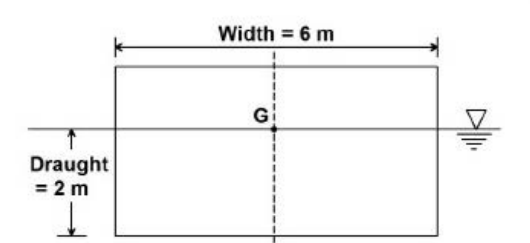
\includegraphics[width=.55\linewidth]{figs/B/fig3.png} 
  \caption{Rectangular Boat}
  \label{B/fig3}
\end{figure}
\hfill\raisebox{-2.5ex}{(GATE 2015 XE)} \\

\vspace{0.2cm}
\begin{enumerate}[label=\alph*)]
\item $-1.0$
\item $0.5$
\item $1.5$
\item $2.0$
\end{enumerate}

\newpage

% Q32
\item Water drains from a large tank through a small orifice at the bottom. If initial water column height is $H$, time to empty is proportional to  
\hfill\raisebox{-2.5ex}{(GATE 2015 XE)} \\

\vspace{0.2cm}
\begin{enumerate}[label=\alph*)]
\item $H^{1/2}$
\item $H$
\item $H^{3/2}$
\item $H^2$
\end{enumerate}
\vspace{0.5cm}

% Q33
\item 2D velocity field $\vec{V} = \pi y \,\mathbf{i} - \pi x\,\mathbf{j}$. A fluid particle initially at $(-1,1)$ has position after unit time:
\vspace{0.2cm}
\hfill\raisebox{-2.5ex}{(GATE 2015 XE)} \\

\begin{enumerate}[label=\alph*)]
\item $(-2,-2)$
\item $(1,-1)$
\item $(1,1)$
\item $(3,-1)$
\end{enumerate}
\vspace{0.5cm}

% Q34 (image: fig4)
\item The figure shows a reducing conduit carrying water. If total head loss due to friction equals loss of potential head between inlet and outlet, $V_2$ in m/s is \_\_\_\_

\begin{figure}[htbp]
  \centering
  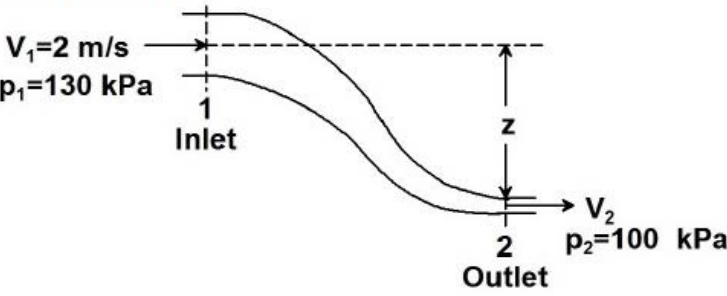
\includegraphics[width=.68\linewidth]{figs/B/fig4.png} 
  \caption{Diagram}
  \label{B/fig4}
\end{figure}
\hfill\raisebox{-2.5ex}{(GATE 2015 XE)} \\

\newpage

% Q35 (image: fig5)
\item A control volume has inflow $i$ and two outflows $o_1$ and $o_2$, with given $\rho, V, A$ for each. The rate of change of mass in the CV (kg/s) is \_\_\_\_
\vspace{0.2cm}

\begin{figure}[htbp]
  \centering
  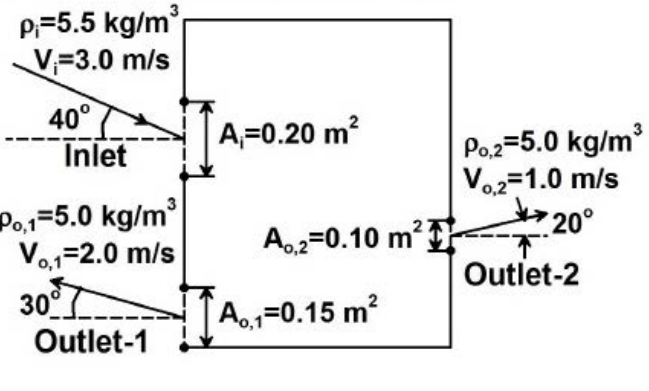
\includegraphics[width=.68\linewidth]{figs/B/fig5.png} 
  \caption{Diagram}
  \label{B/fig5}
\end{figure}
\hfill\raisebox{-2.5ex}{(GATE 2015 XE)} \\

\vspace{0.5cm}

% Q36 (image: fig6)
\item A lawn sprinkler discharges 1 liter/min total. Jet speed at each arm end relative to the arm is $2\pi/30$ m/s, arm length $0.1$ m, frictional torque at pivot $\pi/36$ mN·m. Rotational speed (rpm) is \_\_\_\_

\begin{figure}[htbp]
  \centering
  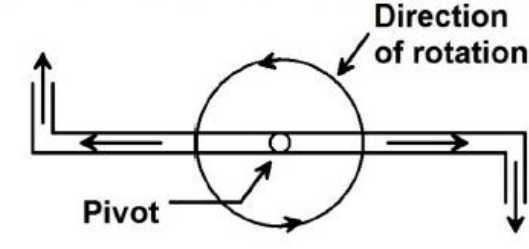
\includegraphics[width=.5\linewidth]{figs/B/fig6.png} 
  \caption{Lawn Sprinkler}
  \label{B/fig6}
\end{figure}
\hfill\raisebox{-2.5ex}{(GATE 2015 XE)} \\

\vspace{0.5cm}

% Q37
\item 2D potential flow field: $V_r = \dfrac{m}{2\pi r}$, $V_\theta = \dfrac{k}{r}$. The stream function $\psi$ with $\psi=0$ at $r=a$, $\theta=0$, is
\vspace{0.05cm}
\hfill\raisebox{-0.5ex}{(GATE 2015 XE)} \\

\begin{enumerate}[label=\alph*)]
\item $\frac{m\theta}{2\pi} + k \ln\dfrac{r}{a}$
\item $\frac{m\theta}{\pi} + k \ln\dfrac{r}{a}$
\item $\frac{m\theta}{2\pi} + \frac{k}{2\pi}\ln\dfrac{r}{a}$
\item $\frac{m\theta}{\pi} + \frac{k}{2\pi}\ln\dfrac{r}{a}$
\end{enumerate}

\newpage

% Q38
\item A steady, inviscid, incompressible 2D flow: $u = ax$, $v = -ay$, gravity along $-y$. Pressure distribution with $p=0$ at origin is
\hfill\raisebox{-2.5ex}{(GATE 2015 XE)} \\

\vspace{0.2cm}
\begin{enumerate}[label=\alph*)]
\item $-\frac{\rho a^2}{2}(x^2+xy+y^2) - \rho gy$
\item $-\frac{\rho a^2}{2}(x^2 - xy + y^2) - \rho gy$
\item $-\frac{\rho a^2}{2}(x^2+y^2) - \rho gy$
\item $-\frac{\rho a^2}{2}(x^2 - y^2) - \rho gy$
\end{enumerate}
\vspace{0.5cm}

% Q39
\item A cylinder radius $0.1$ m rotates clockwise at angular velocity $100/\pi$ rad/s in a cross-flow $10$ m/s, air density $1.2$ kg/m$^3$. The lift force per unit length (N/m) is \_\_\_\_
\hfill\raisebox{-2.5ex}{(GATE 2015 XE)} \\

\vspace{0.5cm}

% Q40
\item Turbulent pipe flow velocity profile: $\displaystyle \frac{u}{u_{max}} = \left(\frac{y}{R}\right)^{1/7}$. Ratio $\dfrac{U_{av}}{U_{max}}$ is  
\hfill\raisebox{-2.5ex}{(GATE 2015 XE)} \\

\vspace{0.2cm}
\begin{enumerate}[label=\alph*)]
\item $\frac{15}{16}$
\vspace{0.1cm}
\item $\frac{49}{60}$
\vspace{0.1cm}
\item $\frac{3}{4}$
\vspace{0.1cm}
\item $\frac{2}{3}$
\end{enumerate}
\vspace{0.5cm}

% Q41
\item A steel sphere ($\rho=7900$ kg/m$^3$) diameter $0.1$ m drops in water ($\rho=1000$ kg/m$^3$), $g=9.81$ m/s$^2$, drag coefficient $1.33$. Terminal velocity (m/s) is \_\_\_\_
\hfill\raisebox{-2.5ex}{(GATE 2015 XE)} \\

\vspace{0.5cm}

% Q42 (image: fig7)
\item An inclined venturimeter with inverted manometer: inlet and throat areas $2\times 10^{-3}$ m$^2$ and $2\times 10^{-4}$ m$^2$; water ($\rho=1000$) and oil ($\rho=800$). Flow rate $Q=5\times 10^{-3}$ m$^3$/s. Neglect viscosity. Manometer reading $h$ (m) is \_\_\_\_

\begin{figure}[htbp]
  \centering
  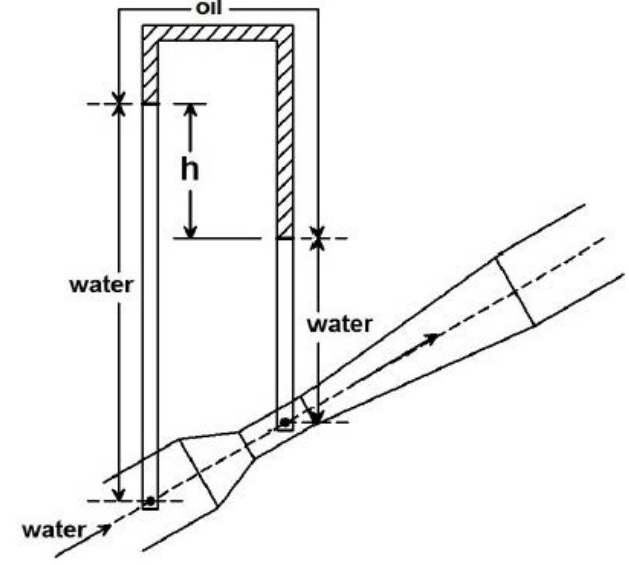
\includegraphics[width=.5\linewidth]{figs/B/fig7.png} 
  \caption{Venturimeter with Inverted Manometer}
  \label{B/fig7}
\end{figure}

\hfill\raisebox{-2.5ex}{(GATE 2015 XE)} \\

\vspace{0.5cm}

% Q43 (image: fig8)
\item A plane jet $Q=0.012$ m$^3$/s, area $6\times 10^{-4}$ m$^2$, strikes a stationary plate inclined at $\theta$, splits into two streams in $3:1$ discharge ratio. Uniform velocities, ignore friction, $\rho=1000$ kg/m$^3$. Magnitude of normal force (N) is \_\_\_\_

\begin{figure}[htbp]
  \centering
  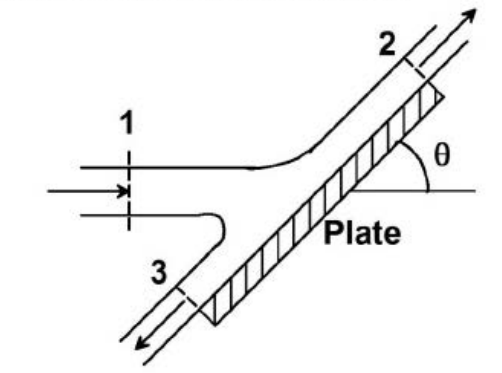
\includegraphics[width=.5\linewidth]{figs/B/fig8.png} 
  \caption{Plate}
  \label{B/fig8}
\end{figure}
\hfill\raisebox{-2.5ex}{(GATE 2015 XE)} \\

\end{enumerate}

\vspace{3\baselineskip}
\begin{center}
    \item[\textbf{END OF SECTION- B}]
\end{center}

%-------SECTION-C-----------------
\newpage

\section*{Materials Science}
\vspace{1cm}

\begin{enumerate}[label=\arabic*)]


% Q44
\item Arrange the following in order of increasing melting point:  
(P) Gallium, (Q) Tungsten, (R) Aluminium, (S) Gold  
\hfill\raisebox{-2.5ex}{(GATE 2015 XE)} \\

\vspace{0.2cm}
\begin{enumerate}[label=\alph*)]
\item P $<$ R $<$ Q $<$ S
\item S $<$ P $<$ R $<$ Q
\item P $<$ R $<$ S $<$ Q
\item R $<$ S $<$ Q $<$ P
\end{enumerate}
\vspace{0.5cm}

% Q45
\item Coordination number of carbon atoms in diamond structure is  
\hfill\raisebox{-2.5ex}{(GATE 2015 XE)} \\

\vspace{0.2cm}
\begin{enumerate}[label=\alph*)]
\item 2
\item 4
\item 6
\item 8
\end{enumerate}
\vspace{0.5cm}

% Q46
\item For an edge dislocation, the Burgers vector is  
\hfill\raisebox{-2.5ex}{(GATE 2015 XE)} \\

\vspace{0.2cm}
\begin{enumerate}[label=\alph*)]
\item parallel to the dislocation line
\item perpendicular to the slip plane
\item perpendicular to the dislocation line
\item parallel to the slip plane
\end{enumerate}
\vspace{0.5cm}

% Q47
\item Hall–Petch relation correlates  
\hfill\raisebox{-2.5ex}{(GATE 2015 XE)} \\

\vspace{0.2cm}
\begin{enumerate}[label=\alph*)]
\item grain size and ductility
\item grain size and strength
\item strength and ductility
\item strength and modulus
\end{enumerate}
\vspace{0.5cm}

% Q48
\item Fatigue failure primarily occurs  
\hfill\raisebox{-2.5ex}{(GATE 2015 XE)} \\

\vspace{0.2cm}
\begin{enumerate}[label=\alph*)]
\item under static loading
\item under cyclic loading
\item under creep conditions
\item above recrystallization temperature
\end{enumerate}
\vspace{0.4cm}

% Q49
\item The eutectoid composition of steel (wt\% C) is  
\hfill\raisebox{-2.5ex}{(GATE 2015 XE)} \\

\vspace{0.2cm}
\begin{enumerate}[label=\alph*)]
\item 0.02
\item 0.8
\item 1.2
\item 2.0
\end{enumerate}
\vspace{0.5cm}

% Q50
\item Which one is NOT a ceramic?  
\hfill\raisebox{-2.5ex}{(GATE 2015 XE)} \\

\vspace{0.2cm}
\begin{enumerate}[label=\alph*)]
\item Alumina
\item Silicon carbide
\item Polyethylene
\item Zirconia
\end{enumerate}
\vspace{0.5cm}

% Q51
\item The electrical conductivity of a pure metal decreases with temperature because
\hfill\raisebox{-2.5ex}{(GATE 2015 XE)} \\

\vspace{0.2cm}
\begin{enumerate}[label=\alph*)]
\item carrier concentration decreases
\item carrier mobility decreases
\item band gap increases
\item lattice constant changes
\end{enumerate}
\vspace{0.5cm}

% Q52
\item The ratio $\rho_{\text{ceramic}}/\rho_{\text{metal}}$ is generally  
\hfill\raisebox{-2.5ex}{(GATE 2015 XE)} \\

\vspace{0.2cm}
\begin{enumerate}[label=\alph*)]
\item $<1$
\item $\approx 1$
\item $>1$
\item $\approx 0.5$
\end{enumerate}
\vspace{0.5cm}

% Q53
\item Compressive strength of ceramics is typically  
\hfill\raisebox{-2.5ex}{(GATE 2015 XE)} \\

\vspace{0.2cm}
\begin{enumerate}[label=\alph*)]
\item higher than tensile strength
\item equal to tensile strength
\item lower than tensile strength
\item unrelated to tensile strength
\end{enumerate}
\vspace{0.5cm}

% Q54
\item The process of heating and slow cooling to remove internal stresses is  \hfill\raisebox{-2.5ex}{(GATE 2015 XE)} \\

\vspace{0.2cm}
\begin{enumerate}[label=\alph*)]
\item hardening
\item tempering
\item annealing
\item quenching
\end{enumerate}
\vspace{0.5cm}

% Q55
\item A polymer with amorphous arrangement is generally  
\hfill\raisebox{-2.5ex}{(GATE 2015 XE)} \\

\vspace{0.2cm}
\begin{enumerate}[label=\alph*)]
\item transparent
\item opaque
\item brittle
\item crystalline
\end{enumerate}

\newpage

% Q56
\item In polymers, increasing crosslinking generally  
\hfill\raisebox{-2.5ex}{(GATE 2015 XE)} \\

\vspace{0.2cm}
\begin{enumerate}[label=\alph*)]
\item increases ductility
\item increases brittleness
\item decreases stiffness
\item decreases glass transition temperature
\end{enumerate}
\vspace{0.5cm}

% Q57
\item The energy gap in a conductor is  
\hfill\raisebox{-2.5ex}{(GATE 2015 XE)} \\

\vspace{0.2cm}
\begin{enumerate}[label=\alph*)]
\item large
\item zero
\item small
\item infinite
\end{enumerate}
\vspace{0.5cm}

% Q58
\item Maximum solid solubility of carbon in $\gamma$-iron at eutectic temperature (wt\% C) is  
\hfill\raisebox{-2.5ex}{(GATE 2015 XE)} \\

\vspace{0.2cm}
\begin{enumerate}[label=\alph*)]
\item 0.02
\item 0.76
\item 2.14
\item 6.67
\end{enumerate}
\vspace{0.5cm}

% Q59
\item Which is a non-ferrous metal?  
\hfill\raisebox{-2.5ex}{(GATE 2015 XE)} \\

\vspace{0.2cm}
\begin{enumerate}[label=\alph*)]
\item Aluminium
\item Steel
\item Cast iron
\item Wrought iron
\end{enumerate}
\vspace{0.5cm}

% Q60
\item Creep in metals occurs predominantly at  
\hfill\raisebox{-2.5ex}{(GATE 2015 XE)} \\

\vspace{0.2cm}
\begin{enumerate}[label=\alph*)]
\item low temperature
\item high temperature
\item room temperature
\item cryogenic temperature
\end{enumerate}
\vspace{0.5cm}

% Q61
\item The Brinell hardness test uses a  
\hfill\raisebox{-2.5ex}{(GATE 2015 XE)} \\

\vspace{0.2cm}
\begin{enumerate}[label=\alph*)]
\item steel ball indenter
\item diamond pyramid
\item cylindrical punch
\item knife edge
\end{enumerate}

\newpage

% Q62
\item The main constituent of glass is  
\hfill\raisebox{-2.5ex}{(GATE 2015 XE)} \\

\vspace{0.2cm}
\begin{enumerate}[label=\alph*)]
\item SiO$_2$
\item Al$_2$O$_3$
\item CaO
\item MgO
\end{enumerate}
\vspace{0.5cm}

% Q63
\item The coordination number in the FCC crystal structure is  
\hfill\raisebox{-2.5ex}{(GATE 2015 XE)} \\

\vspace{0.2cm}
\begin{enumerate}[label=\alph*)]
\item 6
\item 8
\item 12
\item 14
\end{enumerate}
\vspace{0.5cm}

% Q64
\item Polymers with high crystallinity generally have  
\hfill\raisebox{-2.5ex}{(GATE 2015 XE)} \\

\vspace{0.2cm}
\begin{enumerate}[label=\alph*)]
\item higher density
\item lower density
\item same density as amorphous polymers
\item no correlation with density
\end{enumerate}
\vspace{0.5cm}

% Q65
\item The primary strengthening mechanism in precipitation-hardened alloys is
\hfill\raisebox{-2.5ex}{(GATE 2015 XE)} \\

\vspace{0.2cm}
\begin{enumerate}[label=\alph*)]
\item grain boundary strengthening
\item solid solution strengthening
\item dispersion of coherent precipitates
\item work hardening
\end{enumerate}

\end{enumerate}

\vspace{3\baselineskip}
\begin{center}
    \item[\textbf{END OF SECTION- C}]
\end{center}

%-------------------SECTION-D------------------

\newpage
\section*{Thermodynamics}
\vspace{1cm}

\begin{enumerate}[label=\arabic*)]

\item A gas expands following $PV^n = \text{constant}$ from $(P_1,V_1)$ to $V_2 = 2V_1$. For the values of $n$ given below, maximum displacement work is obtained for  
\hfill\raisebox{-2.5ex}{(GATE 2015 XE)} \\

\vspace{0.2cm}
\begin{enumerate}[label=\alph*)]
\item $n = -1$
\item $n = 0$
\item $n = 1$
\item $n = 1.4$
\end{enumerate}
\vspace{0.5cm}

\item A $100\ \Omega$ resistor is heated steadily by passing a current of 20 A. Heating is in surroundings at $30^\circ$C. The rate of increase in entropy of the universe (kW/K) is \_\_\_\_
\hfill\raisebox{-2.5ex}{(GATE 2015 XE)} \\

\vspace{0.5cm}

\item As per Clausius inequality, a system operating on an irreversible cycle transfers  
\hfill\raisebox{-2.5ex}{(GATE 2015 XE)} \\

\vspace{0.2cm}
\begin{enumerate}[label=\alph*)]
\item more entropy to the sink than it receives from the source
\item as much entropy to the sink as it receives from the source
\item less entropy to the sink than it receives from the source
\item less entropy to the sink than that in a reversible cycle
\end{enumerate}
\vspace{0.5cm}

\item The critical point of a substance is the state  
\hfill\raisebox{-2.5ex}{(GATE 2015 XE)} \\

\vspace{0.2cm}
\begin{enumerate}[label=\alph*)]
\item at which the solid, liquid, and vapour phases are in equilibrium
\item beyond which liquid requires very large amount of heat to become vapour
\item beyond which solid sublimates directly to vapour
\item beyond which the distinction between liquid and vapour disappears
\end{enumerate}
\vspace{0.5cm}

\item Sensible cooling of $60\%$ RH air at constant pressure:  
\hfill\raisebox{-2.5ex}{(GATE 2015 XE)} \\

\vspace{0.2cm}
\begin{enumerate}[label=\alph*)]
\item Humidity ratio and relative humidity increase
\item Humidity ratio decreases continuously due to condensation
\item Dry bulb temperature decreases but wet bulb temperature increases
\item Humidity ratio remains constant
\end{enumerate}
\vspace{0.5cm}

\item The COP of a reversible refrigerator operating between two reservoirs is $4.0$. The efficiency (\%) of a reversible heat engine operating between the same limits is \_\_\_\_
\hfill\raisebox{-2.5ex}{(GATE 2015 XE)} \\

\newpage

\item For a real superheated vapour (non-ideal gas), the differential change in specific enthalpy is given by  
\hfill\raisebox{-2.5ex}{(GATE 2015 XE)} \\

\vspace{0.2cm}
\begin{enumerate}[label=\alph*)]
\item $dh = C_p\,dT$
\item $dh = C_p\,dT + \frac{\partial h}{\partial v} dv$
\item $dh = C_p\,dT + \frac{\partial h}{\partial p} dp$
\item $dh = C_p\,dT + \frac{\partial p}{\partial T} dp$
\end{enumerate}
\vspace{0.5cm}

\item An ideal gas mixture O$_2$ (MW=32) and CO$_2$ (MW=44) has 40\% and 60\% mass composition respectively. Total pressure is $200$ kPa. The partial pressure of O$_2$ (kPa) is \_\_\_\_
\hfill\raisebox{-2.5ex}{(GATE 2015 XE)} \\

\vspace{0.5cm}

\item For an ideal Rankine cycle, increasing the superheat of steam at boiler exit will 
\hfill\raisebox{-2.5ex}{(GATE 2015 XE)} \\

\vspace{0.2cm}
\begin{enumerate}[label=\alph*)]
\item decrease net work output
\item increase cycle efficiency
\item decrease cycle efficiency
\item decrease quality of steam at turbine exit
\end{enumerate}
\vspace{0.5cm}

\item Two moles of air at 1 atm, $21.1^\circ$C pass into an adiabatic device and separate into a hot stream (0.4 mol, $176.3^\circ$C) and a cold stream (1.6 mol, $-17.7^\circ$C), all at 1 atm. Which statement is correct? 
\vspace{0.2cm}
\hfill\raisebox{-2.5ex}{(GATE 2015 XE)} \\

\begin{enumerate}[label=\alph*)]
\item Total entropy change is zero
\item Total entropy change is positive
\item Device violates Second Law
\item Device violates First Law
\end{enumerate}
\vspace{0.5cm}

\item For a real gas through a porous plug with coefficient $\alpha$, Joule–Thomson cooling is observed when
\vspace{0.2cm}
\hfill\raisebox{-2.5ex}{(GATE 2015 XE)} \\

\begin{enumerate}[label=\alph*)]
\item $0 < \alpha T < 1$
\item $\alpha T = 1$
\item $\alpha T > 1$
\item $\alpha T = 0$
\end{enumerate}
\vspace{0.5cm}

\item A lead bullet at $100^\circ$C, moving at $500$ m/s strikes a target and stops adiabatically. $c_p=92$ J/kg°C, melt point $327.5^\circ$C, $L=108$ kJ/kg. The percentage of mass melted is \_\_\_\_
\hfill\raisebox{-2.5ex}{(GATE 2015 XE)} \\

\vspace{0.5cm}

\item Air–water vapour mixture, 100 m$^3$ at $p=100$ kPa, $T=35^\circ$C, RH=75\%, $p_{sat}$=5.63 kPa. Mass of water vapour (kg) = \_\_\_\_
\hfill\raisebox{-2.5ex}{(GATE 2015 XE)} \\

\newpage

\item 1 kg ideal gas at $T=1200$ K, $C_v=718$ J/kgK in rigid vessel, ambient 300 K. Maximum work (kJ) obtainable =  
\hfill\raisebox{-2.5ex}{(GATE 2015 XE)} \\

\vspace{0.2cm}
\begin{enumerate}[label=\alph*)]
\item 646.2
\item 484.7
\item 387.7
\item 347.6
\end{enumerate}
\vspace{0.5cm}

\item Boiling point of water changes from $99.62^\circ$C at 1 bar to $105.99^\circ$C at 1.25 bar. Boiling point at 1.5 bar is \_\_\_\_
\hfill\raisebox{-2.5ex}{(GATE 2015 XE)} \\

\vspace{0.5cm}

\item Ideal gas expands adiabatically in a frictionless nozzle from 31 bar, 800 K to 1 bar. $C_p=1$ kJ/kgK, $\gamma=1.4$, neglect inlet kinetic energy. Exit velocity (m/s) =  
\hfill\raisebox{-2.5ex}{(GATE 2015 XE)} \\

\vspace{0.2cm}
\begin{enumerate}[label=\alph*)]
\item 32
\item 500
\item 707
\item 1000
\end{enumerate}
\vspace{0.5cm}

\item One kmol H$_2$ ($\gamma=1.4$) mixes with one kmol N$_2$ ($\gamma=1.4$), both at 1 bar, 300 K, in an adiabatic vessel. Final mixture at 1 bar, 300 K. Entropy change (kJ/K) =  
\hfill\raisebox{-2.5ex}{(GATE 2015 XE)} \\

\vspace{0.2cm}
\begin{enumerate}[label=\alph*)]
\item $-5.76$
\item 0
\item 5.76
\item 11.53
\end{enumerate}
\vspace{0.5cm}

\item A cycle 1–2 constant pressure expansion, 2–3 reversible adiabatic expansion, 3–1 irreversible adiabatic compression. Which is true?  
\hfill\raisebox{-2.5ex}{(GATE 2015 XE)} \\

\vspace{0.2cm}
\begin{enumerate}[label=\alph*)]
\item Net work = 0 (no heat transfer)
\item Feasible and net positive work
\item Impossible by Kelvin–Planck statement
\item Impossible by First Law
\end{enumerate}
\vspace{0.5cm}

\item 1 kg saturated liquid–vapour water at 150 kPa ($u_f=467$ kJ/kg, $v_f=0.001053$ m$^3$/kg; $u_g=2520$ kJ/kg, $v_g=1.159$ m$^3$/kg), quality $x=0.7$, is heated at constant pressure with paddle wheel work input =50 kJ, final state = saturated vapour. Heat added (kJ) = \_\_\_\_
\hfill\raisebox{-2.5ex}{(GATE 2015 XE)} \\

\vspace{0.5cm}

\item A 2 kg metal block at 500 K is brought into contact with a 5 kg metal block at 300 K in an insulated environment until equilibrium is reached. Both metals have $C_p=0.4$ kJ/kgK. Entropy change of the universe (kJ/K) = \_\_\_\_
\hfill\raisebox{-2.5ex}{(GATE 2015 XE)} \\

\vspace{0.5cm}

\item A rigid insulated tank is divided into two equal parts by a partition. One side contains air at 800 kPa, 350 K, the other side is a vacuum. The partition is removed. Final temperature (K) = \_\_\_\_
\vspace{0.2cm}
\hfill\raisebox{-2.5ex}{(GATE 2015 XE)} \\

\end{enumerate}

\vspace{3\baselineskip}
\begin{center}
    \item[\textbf{END OF SECTION- D}]
\end{center}

%----------------------SECTION-E-----------------------------
\newpage
\section*{Polymer Science}
\vspace{1cm}
\begin{enumerate}[label=\arabic*)]

\item The biodegradable polymer among the following polymers is
\hfill\raisebox{-2.5ex}{(GATE 2015 XE)} \\

\vspace{0.2cm}
\begin{enumerate}[label=\alph*)]
\item poly(lactic acid)
\item poly(butylene terephthalate)
\item polystyrene
\item polypropylene
\end{enumerate}

\vspace{0.5cm}

\item Notched impact strength of a plastic decreases with
\hfill\raisebox{-2.5ex}{(GATE 2015 XE)} \\

\vspace{0.2cm}
\begin{enumerate}[label=\alph*)]
\item increase in notch tip radius
\item increase in notch depth
\item increase in temperature
\item decrease in notch depth
\end{enumerate}

\vspace{0.5cm}

\item The compound used as a reactive diluent in unsaturated polyester resins is
\hfill\raisebox{-2.5ex}{(GATE 2015 XE)} \\

\vspace{0.2cm}
\begin{enumerate}[label=\alph*)]
\item benzene
\item cresol
\item styrene
\item adipic acid
\end{enumerate}

\vspace{0.5cm}

\item The diameter of a die of an extruder producing extrudate of diameter 2.4 mm with a die-swell ratio of 2 is \_\_\_\_ mm.
\hfill\raisebox{-2.5ex}{(GATE 2015 XE)} \\
\vspace{0.5cm}

\item The degree of polymerization of Nylon 6 (ignore end-groups) with molar mass of 1,00,000 g mol$^{-1}$ is \_\_\_\_
\hfill\raisebox{-2.5ex}{(GATE 2015 XE)} \\

\vspace{0.5cm}

\item Ring opening polymerization is used for the synthesis of
\hfill\raisebox{-2.5ex}{(GATE 2015 XE)} \\

\vspace{0.2cm}
\begin{enumerate}[label=\alph*)]
\item Nylon 6
\item poly(acrylic acid)
\item Nylon 66
\item poly(ethylene terephthalate)
\end{enumerate}

\newpage 

\item Which among the following are used as initiators for free radical polymerization?

P. $K_2SO_4$  Q. $K_2S_2O_8$ \\
R. AlBN  S.t-butyl Hydroperoxide + $Fe^{2+}$

 \hfill\raisebox{-2.5ex}{(GATE 2015 XE)} \\
 
\vspace{0.2cm}
\begin{enumerate}[label=\alph*)]
\item P, Q \& S only
\item Q, R \& S only
\item P, R \& S only
\item P, Q \& R only
\end{enumerate}

\vspace{0.5cm}

\item Weight average molecular weight can be determined by
\hfill\raisebox{-2.5ex}{(GATE 2015 XE)} \\

\vspace{0.2cm}
\begin{enumerate}[label=\alph*)]
\item Osmometry
\item Ebullimetry
\item End group analysis
\item Light scattering
\end{enumerate}

\vspace{0.5cm}

\item Butyl rubber is a copolymer of
\hfill\raisebox{-2.5ex}{(GATE 2015 XE)} \\

\vspace{0.2cm}
\begin{enumerate}[label=\alph*)]
\item isobutylene and butadiene
\item butadiene and 1-butene
\item isobutylene and isoprene
\item isoprene and 1-butene
\end{enumerate}

\vspace{0.5cm}

\item Match the characterization technique with the polymer property it is used to determine.
\hfill\raisebox{-2.5ex}{(GATE 2015 XE)} \\

\begin{center}
\begin{tabular}{ll}
    \textbf{Group I} & \textbf{Group II} \\
    P. Ferrite & 1. Hexagonal Close Packed (HCP) \\
    Q. Austenite & 2. Body Centered Cubic (BCC) \\
    R. Martensite & 3. Body Centered Tetragonal (BCT) \\
    & 4. Face Centered Cubic (FCC)
\end{tabular}
\end{center}

\hfill\raisebox{-2.5ex}{(GATE 2015 XE)} \\

\vspace{0.2cm}
\begin{enumerate}[label=\alph*)]
\item P–3, Q–1, R–4, S–2
\item P–3, Q–4, R–2, S–1
\item P–2, Q–4, R–1, S–3
\item P–2, Q–1, R–4, S–3
\end{enumerate}

\newpage

\item Match the following plastic additives with their function.

\begin{tabular}{|c|c|c|}
     \hline
     \textbf{Mineral} & \textbf{Modal abundance \brak{\%}} & \textbf{Partition coefficient}\\
     \hline
     Clinopyroxene & $45$ & $0.506$ \\
      \hline
      Orthopyroxene & $40$ & $0.42$ \\
      \hline
      Olivine & $10$ & $0.045$ \\
      \hline
      Plagioclase & $05$ & $0.019$ \\
      \hline
\end{tabular}

\hfill\raisebox{-2.5ex}{(GATE 2015 XE)} \\

\vspace{0.2cm}
\begin{enumerate}[label=\alph*)]
\item P–2; Q–4; R–1; S–3
\item P–4; Q–1; R–3; S–2
\item P–2; Q–1; R–4; S–3
\item P–3; Q–1; R–4; S–2
\end{enumerate}

\vspace{0.5cm}

\item The correct statement with respect to electrical property of polymeric materials is
\hfill\raisebox{-2.5ex}{(GATE 2015 XE)} \\

\vspace{0.2cm}
\begin{enumerate}[label=\alph*)]
\item For non polar materials, dielectric constant is independent of frequency \& temperature
\item For polar materials, dielectric constant depends on frequency but not on temperature
\item For non polar materials, power losses are high and depend on temperature \& frequency
\item For polar materials, power losses are low and independent of frequency
\end{enumerate}

\vspace{0.5cm}

\item The order of melting point for the given polymers is
\hfill\raisebox{-2.5ex}{(GATE 2015 XE)} \\

\vspace{0.2cm}
\begin{enumerate}[label=\alph*)]
\item Nylon 66 $>$ PTFE $>$ Nylon 6 $>$ PP
\item Nylon 66 $>$ Nylon 6 $>$ PTFE $>$ PP
\item PTFE $>$ Nylon 66 $>$ Nylon 6 $>$ PP
\item PTFE $>$ Nylon 6 $>$ Nylon 66 $>$ PP
\end{enumerate}

\vspace{0.5cm}

\item Match the processing technique used to manufacture the appropriate product.

\begin{table}[htbp]
  \centering
  \caption{Table-3}
  \label{table3}
  \begin{tabular}{cc}
  \textbf{Processing Technique} & \textbf{Producct} \\ \\
    P. Calendering & 1. Pipes \\
    Q. Extrusion & 2. Disposable cups \\
    R. Injection moulding & 3. Sheets \\
    S. Thermoforming & 4. Nylon gears \\
  \end{tabular}
\end{table}

\hfill\raisebox{-2.5ex}{(GATE 2015 XE)} \\

\vspace{0.2cm}
\begin{enumerate}[label=\alph*)]
\item P–3; Q–2; R–1; S–4
\item P–3; Q–1; R–2; S–4
\item P–3; Q–1; R–4; S–2
\item P–3; Q–2; R–4; S–1
\end{enumerate}

\newpage

\item Match the thermosetting resins to the raw materials they are synthesized from.

\begin{center}
\begin{tabular}{|c|c|c|}
    \hline
    Task & Task time (Seconds) & Immediate predecessor(s) \\
    \hline
    P & 20 & - \\ \hline
    Q & 25 & P \\  \hline
    R & 10 & Q \\ \hline
    S & 15 & Q \\ \hline 
    T & 25 & R, S \\    \hline
\end{tabular}
\end{center}

\hfill\raisebox{-2.5ex}{(GATE 2015 XE)} \\

\vspace{0.2cm}
\begin{enumerate}[label=\alph*)]
\item P–4; Q–2; R–3; S–1
\item P–3; Q–1; R–2; S–4
\item P–3; Q–2; R–1; S–4
\item P–3; Q–1; R–4; S–2
\end{enumerate}

\vspace{0.5cm}

\item The damping factor of a solid polymer under sinusoidal loading in single cantilever mode showing 80 percent recovery in modulus is \_\_\_\_
\hfill\raisebox{-2.5ex}{(GATE 2015 XE)} \\
\vspace{0.5cm}

\item A styrene–butadiene random copolymer with equal weight fraction of polystyrene ($T_g=100^\circ$C) and polybutadiene ($T_g=-100^\circ$C) shows a single glass transition peak. The $T_g$ of the copolymer is \_\_\_\_ $^\circ$C.
\hfill\raisebox{-2.5ex}{(GATE 2015 XE)} \\
\vspace{0.5cm}

\item In a unidirectional carbon fibre reinforced epoxy composite, the ratio of fibre-to-matrix moduli is 30 and the fibres take up 50\% of the cross-section. The percentage of applied force taken up by the fibres is \_\_\_\_
\hfill\raisebox{-2.5ex}{(GATE 2015 XE)} \\

\vspace{0.5cm}

\item The viscoelastic behavior of a plastic is represented by spring and dashpot elements having constants of 2 GN m$^{-2}$ and 90 GN s m$^{-2}$, respectively. If a constant stress of 12 MN m$^{-2}$ is applied, the strain predicted by Maxwell model after 50 s is \_\_\_\_ \%
\hfill\raisebox{-2.5ex}{(GATE 2015 XE)} \\

\vspace{0.5cm}
\newpage

\item Match the elastomers given below to their suitable application.

\begin{table}[h!]
\centering
\begin{tabular}{|c|c|c|c|}
\hline
\textbf{Pressure} & \textbf{Temperature} & \multicolumn{2}{c|}{\textbf{Specific enthalpy}} \\ \cline{3-4} 
\textbf{(kPa)} & \textbf{($^\circ$C)} & $h_f$ (kJ/kg) & $h_g$ (kJ/kg) \\ \hline
150.9 & $-20$ & 17.82 & 178.74 \\ \hline
500 & 15.6 & 50.64 & 195.01 \\ \hline
\end{tabular}
\end{table}

\hfill\raisebox{-2.5ex}{(GATE 2015 XE)} \\

\vspace{0.2cm}
\begin{enumerate}[label=\alph*)]
\item P–3; Q–4; R–2; S–1
\item P–4; Q–3; R–2; S–1
\item P–3; Q–2; R–4; S–1
\item P–1; Q–4; R–2; S–3
\end{enumerate}


\item Match the following reagents to their function in natural rubber latex technology.

\begin{table}[htbp]
  \centering
  \caption{Table-6}
  \label{tab:tables/table6.tex}
  \begin{tabular}{cc}
  \textbf{Reagent} & \textbf{Function} \\ \\
    P.Ammonia  & 1. Prevent storage hardening \\
    Q. Hydroxylamine & 2. Delay plugging mechanism \\
    R. Formic acid & 3. Stabilizer \\
    S. Ethephone & 4. Coagulating agent \\
  \end{tabular}
\end{table}

\hfill\raisebox{-2.5ex}{(GATE 2015 XE)} \\

\vspace{0.2cm}
\begin{enumerate}[label=\alph*)]
\item P–3; Q–1; R–2; S–4
\item P–3; Q–2; R–4; S–1
\item P–3; Q–1; R–4; S–2
\item P–3; Q–4; R–1; S–2
\end{enumerate}

\vspace{0.5cm}

\item 1.0 g of a polybutadiene sample with carboxylic acid groups at both the ends requires 2.5 mL of 0.1 M KOH for complete neutralization. The molecular weight of the polymer in g mol$^{-1}$ is \_\_\_\_
\vspace{0.5cm}
\hfill\raisebox{-2.5ex}{(GATE 2015 XE)} \\



\end{enumerate}

\vspace{2\baselineskip}
\begin{center}
    \item[\textbf{END OF SECTION- E}]
\end{center}


%--------------SECTION-F---------------

\newpage
\section*{Food Technology}
\vspace{1cm}
\begin{enumerate}[label=\arabic*)]

\item Standard pasteurization protocol for milk is adequate for destroying
\hfill\raisebox{-2.5ex}{(GATE 2015 XE)} \\

\vspace{0.2cm}
\begin{enumerate}[label=\alph*)]
\item \textit{Clostridium sporogenes}
\item \textit{Bacillus cereus}
\item \textit{Clostridium botulinum}
\item \textit{Listeria monocytogenes}
\end{enumerate}

\vspace{0.5cm}

\item Which one of the following is NOT a component of an evaporator?
\hfill\raisebox{-2.5ex}{(GATE 2015 XE)} \\

\vspace{0.2cm}
\begin{enumerate}[label=\alph*)]
\item Heat exchanger
\item Vacuum separator
\item Condenser
\item Cyclone separator
\end{enumerate}

\vspace{0.5cm}

\item Among the following animal foods, the fat content is least in
\hfill\raisebox{-2.5ex}{(GATE 2015 XE)} \\

\vspace{0.2cm}
\begin{enumerate}[label=\alph*)]
\item Beef
\item Chicken meat
\item Pork
\item Lamb flesh
\end{enumerate}

\vspace{0.5cm}

\item The enzyme that hydrolyzes starch to maltose is
\hfill\raisebox{-2.5ex}{(GATE 2015 XE)} \\

\vspace{0.2cm}
\begin{enumerate}[label=\alph*)]
\item $\alpha$-amylase
\item $\beta$-amylase
\item glucoamylase
\item cyclodextrin glucanotransferase
\end{enumerate}

\vspace{0.5cm}

\item Which one of the following is NOT enriched in endosperm during parboiling of paddy?
\hfill\raisebox{-2.5ex}{(GATE 2015 XE)} \\

\vspace{0.2cm}
\begin{enumerate}[label=\alph*)]
\item Thiamine
\item Niacin
\item Iron
\item Fat
\end{enumerate}

\newpage

\item Heat-treated legume seed proteins are more digestible than those of untreated legume seed proteins due to
\hfill\raisebox{-2.5ex}{(GATE 2015 XE)} \\

\vspace{0.2cm}
\begin{enumerate}[label=\alph*)]
\item reaction of reducing sugars with $\varepsilon$-amino group of lysine
\item increased binding of lectins to intestinal mucosal cells
\item thermolabile nature of lectins and Kunitz-type protease inhibitors
\item thermolabile nature of Bowman–Birk type of inhibitor
\end{enumerate}

\vspace{0.5cm}

\item What is the percent relative humidity at which both the dry bulb and wet bulb thermometers would record equal temperatures?
\hfill\raisebox{-2.5ex}{(GATE 2015 XE)} \\

\vspace{0.2cm}
\begin{enumerate}[label=\alph*)]
\item 0
\item 10
\item 50
\item 100
\end{enumerate}

\vspace{0.5cm}

\item How many fold would the g-number of a centrifuge increase by doubling both the spinning speed and bowl diameter?
\hfill\raisebox{-2.5ex}{(GATE 2015 XE)} \\

\vspace{0.2cm}
\begin{enumerate}[label=\alph*)]
\item 2
\item 4
\item 8
\item 16
\end{enumerate}

\vspace{0.5cm}

\item The gradual decrease in viscosity of tomato paste during storage can be prevented by quickly heating it to $82^\circ$C, because
\hfill\raisebox{-2.5ex}{(GATE 2015 XE)} \\

\vspace{0.2cm}
\begin{enumerate}[label=\alph*)]
\item water soluble pectin interacts with calcium
\item hemicellulose prevents decrease in viscosity
\item lignin prevents decrease in viscosity
\item pectin methyl esterase is inactivated
\end{enumerate}

\vspace{0.5cm}

\item Match the enzyme in Group I with its corresponding application in Group II.

\begin{table}[htbp]
  \centering
  \caption{Table-7}
  \label{tab:tables/table7.tex}
  \begin{tabular}{cc}
\textbf{Additives} & \textbf{Fuction}\\

P. Molybdenum disulphide & 1. Heat stabilizer \\
Q. Glycerol monostearate & 2. UV-absorber \\
R. Tribasic lead sulphate & 3. Antistatic agent \\
S. 2-hydroxybenzophenone & 4. Solid layer lubricant \\
  
  
  
  \end{tabular}
\end{table}

\hfill\raisebox{-0.5ex}{(GATE 2015 XE)} \\

\vspace{0.05cm}
\begin{enumerate}[label=\alph*)]
\item P–2, Q–1, R–4, S–3
\item P–3, Q–1, R–4, S–2
\item P–1, Q–2, R–3, S–4
\item P–4, Q–3, R–2, S–1
\end{enumerate}

\newpage

\item Milk is flowing at $0.12\ \mathrm{m^3,min^{-1}}$ in a $2.5$ cm diameter pipe. The temperature of the milk is $21^\circ$C and the corresponding viscosity and density are $2.1\times 10^{-3}\ \mathrm{Pa,s}$ and $1029\ \mathrm{kg,m^{-3}}$, respectively. If the flow is found to be turbulent under the given conditions, the Reynolds number is \_\_\_\_
\hfill\raisebox{-2.5ex}{(GATE 2015 XE)} \\

\vspace{0.5cm}

\item Whole milk (34,950 kg) containing 4\% fat is to be separated in 6 h period into skim milk with 0.45\% fat and cream with 45\% fat. The flow rate of cream stream (kg/h) from the separator is \_\_\_\_
\vspace{0.2cm}
\hfill\raisebox{-2.5ex}{(GATE 2015 XE)} \\

\vspace{0.5cm}

\item Match the edible plant tissue in Group I with the type of carotenoid given in Group II.

\begin{table}[htbp]
  \centering
  \caption{Table-8}
  \label{table8}
  \begin{tabular}{cc}
  \textbf{Group-I} & \textbf{Group-II} \\ \\
    P. Corn & 1. Lycopene \\
    Q. Red pepper & 2. $\beta$-Carotene \\
    R. Pumpkin & 3. Capsanthin \\
    S. Tomato & 4. Lutein \\
  \end{tabular}
\end{table}

\hfill\raisebox{-2.5ex}{(GATE 2015 XE)} \\

\vspace{0.2cm}
\begin{enumerate}[label=\alph*)]
\item P–4, Q–3, R–2, S–1
\item P–2, Q–4, R–3, S–1
\item P–3, Q–4, R–2, S–1
\item P–4, Q–1, R–2, S–3
\end{enumerate}

\vspace{0.5cm}

\item Undesirable bitterness frequently encountered in cured cheese is due to the
\hfill\raisebox{-2.5ex}{(GATE 2015 XE)} \\

\vspace{0.2cm}
\begin{enumerate}[label=\alph*)]
\item presence of naringen
\item formation of limonin
\item overall hydrophobicity of amino acid side-chains in peptide
\item conversion of humulone to isohumulone
\end{enumerate}

\vspace{0.5cm}

\item Green tea is considered to be a more healthy option than black tea because it
\hfill\raisebox{-2.5ex}{(GATE 2015 XE)} \\

\vspace{0.2cm}
\begin{enumerate}[label=\alph*)]
\item has high content of polyphenols
\item is richer in thearubigin
\item does not require any sweetener during tea preparation
\item has no microbial load
\end{enumerate}

\vspace{0.5cm}

\item Multiple effect evaporation leads to
\hfill\raisebox{-2.5ex}{(GATE 2015 XE)} \\

\vspace{0.2cm}
\begin{enumerate}[label=\alph*)]
\item reduction in operating cost and reduction in capital cost
\item increase in operating cost and increase in capital cost
\item increase in operating cost and reduction in capital cost
\item reduction in operating cost and increase in capital cost
\end{enumerate}

\newpage

\item A dilute pineapple juice is heated in a double pipe heat exchanger from $28^\circ$C to $75^\circ$C by heat exchanging with hot water flowing in shell in counter current direction. Hot water is entering the shell at $95^\circ$C and leaving at $85^\circ$C. The log mean temperature difference ($^\circ$C) is\ \_\_\_\_
\hfill\raisebox{-2.5ex}{(GATE 2015 XE)} \\

\vspace{0.5cm}

\item Heat is transferred by radiation to a loaf of bread in an oven at a uniform temperature of $177^\circ$C. The total surface area and temperature of the loaf are $0.0645\ \mathrm{m^2}$ and $100^\circ$C, respectively. The surface emissivity of the loaf is $0.85$ and the value of Stefan–Boltzmann constant is $5.67\times 10^{-8}\ \mathrm{W,m^{-2},K^{-4}}$. The net heat transfer (W) is \_\_\_\_
\hfill\raisebox{-2.5ex}{(GATE 2015 XE)} \\

\vspace{0.5cm}

\item Granulated sugar, having an average particle size of $500\ \mu$m, is milled to produce icing sugar having an average particle size of $25\ \mu$m. The power requirement was $10$ kW as obtained by Rittinger’s law. If the same mill were to be used to produce fondant sugar having an average particle size of $20\ \mu$m at the same capacity, the power requirement (kW) would be \_\_\_\_
\hfill\raisebox{-2.5ex}{(GATE 2015 XE)} \\

\vspace{0.5cm}

\item One ton of soybean containing 18\% oil, 35\% protein, 27.1\% carbohydrates, 9.4\% of fibre and ash, and 10.5\% moisture is crushed and pressed. The residual oil content in the pressed cake is 6\%. Assuming that there is no loss of protein and water with oil, the amount of oil (kg) obtained from the crusher is \_\_\_\_
\hfill\raisebox{-2.5ex}{(GATE 2015 XE)} \\

\vspace{0.5cm}

\item Match the processing method in Group I with the operation carried out in Group II.

\begin{table}[htbp]
  \centering
  \caption{Table-9}
  \label{tab:tables/table9.tex}
  \begin{tabular}{cc}
  \textbf{Group-I} & \textbf{Group-II} \\ \\
    P. Degumming & 1. Crystallization of triacylglycerol by cooling to remove fat crystals \\
    Q. Deacidifying & 2. Passing heated oil over charcoal \\
    R. Bleaching & 3. Using alkaline solution to remove fatty acids \\
    S. Winterizing & 4. Wetting with water to remove lecithin \\
  \end{tabular}
\end{table}

\hfill\raisebox{-2.5ex}{(GATE 2015 XE)} \\

\begin{enumerate}[label=\alph*)]
\item P–3, Q–1, R–4, S–2
\item P–4, Q–3, R–1, S–2
\item P–4, Q–3, R–2, S–1
\item P–3, Q–1, R–2, S–4
\end{enumerate}

\vspace{0.5cm}

\item The order of succession of microbes in the spoilage of milk, involving (P) \textit{Lactobacillus}, (Q) protein digesting bacteria, (R) \textit{Lactococcus lactis}, (S) yeasts and molds, is
\hfill\raisebox{-2.5ex}{(GATE 2015 XE)} \\

\vspace{0.05cm}
\begin{enumerate}[label=\alph*)]
\item S $>$ R $>$ Q $>$ P
\item S $>$ Q $>$ R $>$ P
\item R $>$ P $>$ S $>$ Q
\item Q $>$ S $>$ P $>$ R
\end{enumerate}


\end{enumerate}

\vspace{0.35cm}
\begin{center}
    \item[\textbf{END OF SECTION- F}]
\end{center}


\end{document}
